\mfpicnumber{1}

\opengraphsfile{IntrotoFunctions}

\setcounter{footnote}{0}

\label{IntrotoFunctions}

One of the core concepts in College Algebra is the \textbf{function}.  There are many ways to describe a function and we begin by defining a function as a special kind of relation.

\medskip

\colorbox{ResultColor}{\bbm

%\smallskip

\begin{defn}

\label{functiondefn}

A relation in which each $x$-coordinate is matched with only one $y$-coordinate is said to describe $y$ as a \index{function ! definition as a relation} \textbf{function} of $x$.

\end{defn}

\ebm}

\medskip

\begin{ex}  Which of the following relations describe $y$ as a function of $x$?

\begin{multicols}{2}

\begin{enumerate}

\item  $R_{\mbox{\tiny$1$}} = \{ (-2,1), (1,3), (1,4), (3,-1) \}$

\item  $R_{\mbox{\tiny$2$}} = \{ (-2,1), (1,3), (2,3), (3,-1) \}$

\end{enumerate}

\end{multicols}

\smallskip

{\bf Solution.}  A quick scan of the points in $R_{\mbox{\tiny$1$}}$ reveals that the $x$-coordinate $1$ is matched with two \emph{different} $y$-coordinates:  namely $3$ and $4$.  Hence in $R_{\mbox{\tiny$1$}}$, $y$ is not a function of $x$.  On the other hand, every $x$-coordinate in $R_{\mbox{\tiny$2$}}$ occurs only once which means each $x$-coordinate has only one corresponding $y$-coordinate.  So, $R_{\mbox{\tiny$2$}}$  does represent $y$ as a function of $x$.  \qed

\end{ex}

\smallskip

Note that in the previous example, the relation $R_{\mbox{\tiny$2$}}$ contained two different points with the same $y$-coordinates, namely $(1,3)$ and $(2,3)$. Remember, in order to say $y$ is a function of $x$, we just need to ensure the same $x$-coordinate isn't used in more than one point.\footnote{We will have occasion later in the text to concern ourselves with the concept of $x$ being a function of $y$.  In this case, $R_{\mbox{\tiny$1$}}$ represents $x$ as a function of $y$;  $R_{\mbox{\tiny$2$}}$ does not.} 

\smallskip

To see what the function concept means geometrically, we graph $R_{\mbox{\tiny$1$}}$ and $R_{\mbox{\tiny$2$}}$ in the plane.

\medskip

\hspace{1in} \begin{tabular}{m{2.55in}m{2.55in}}

\begin{mfpic}[15]{-3}{4}{-2}{5}
\point[4pt]{ (-2,1), (1,3), (1,4), (3,-1) }
\axes
\tlabel[cc](4,-0.5){\scriptsize $x$}
\tlabel[cc](0.5,5){\scriptsize $y$}
\xmarks{-2 step 1 until 3 }
\ymarks{-1 step 1 until 4}
\tcaption{The graph of $R_{\mbox{\tiny$1$}}$}
\tlpointsep{5pt}
\scriptsize
\axislabels {x}{{$-2 \hspace{7pt}$} -2, {$-1 \hspace{7pt}$} -1, {$1$} 1, {$2$} 2, {$3$} 3}
\axislabels {y}{{$-1$} -1, {$1$} 1, {$2$} 2, {$3$} 3, {$4$} 4}
\normalsize
\end{mfpic}  & 
\begin{mfpic}[15]{-3}{4}{-2}{5}
\point[4pt]{ (-2,1), (1,3), (2,3), (3,-1)}
\axes
\tlabel[cc](4,-0.5){\scriptsize $x$}
\tlabel[cc](0.5,5){\scriptsize $y$}
\xmarks{-2 step 1 until 3 }
\ymarks{-1 step 1 until 4}
\tcaption{The graph of $R_{\mbox{\tiny$2$}}$}
\tlpointsep{5pt}
\scriptsize
\axislabels {x}{{$-2 \hspace{7pt}$} -2, {$-1 \hspace{7pt}$} -1, {$1$} 1, {$2$} 2, {$3$} 3}
\axislabels {y}{{$-1$} -1, {$1$} 1, {$2$} 2, {$3$} 3, {$4$} 4}
\normalsize
\end{mfpic}  \\

\end{tabular}

\smallskip

The fact that the $x$-coordinate $1$ is matched with two different $y$-coordinates in $R_{\mbox{\tiny$1$}}$ presents itself graphically as the points $(1,3)$ and $(1,4)$ lying on the same vertical line, $x=1$.  If we turn our attention to the graph of $R_{\mbox{\tiny$2$}}$, we see that no two points of the relation lie on the same vertical line.  We can generalize this idea as follows

\medskip

\colorbox{ResultColor}{\bbm

%\smallskip

\begin{thm}  \textbf{\index{Vertical Line Test (VLT)}The Vertical Line Test:}  A set of points in the plane represents $y$ as a function of $x$ if and only if no two points lie on the same vertical line.

\label{VLT}

\end{thm}

\ebm}

\pagebreak

It is worth taking some time to meditate on the Vertical Line Test; it will check to see how well you understand the concept of `function' as well as the concept of `graph'.

\begin{ex}  Use the Vertical Line Test to determine which of the following relations describes $y$ as a function of $x$.

\begin{center}

\begin{tabular}{cc}

\begin{mfpic}[20]{-1}{4}{-2}{5}
\circle{(2,2),1}
\axes
\tlabel[cc](4,-0.5){\scriptsize $x$}
\tlabel[cc](0.5,5){\scriptsize $y$}
\xmarks{1 step 1 until 3 }
\ymarks{-1 step 1 until 4}
\tcaption{The graph of $R$}
\tlpointsep{5pt}
\scriptsize
\axislabels {x}{{$1$} 1, {$2$} 2,  {$3$} 3}
\axislabels {y}{{$-1$} -1, {$1$} 1, {$2$} 2,  {$3$} 3, {$4$} 4}
\normalsize
\end{mfpic} \hspace{1.5in}

& 

\begin{mfpic}[20]{-3}{3}{-2}{5}
\arrow\function{-1.5,2,0.1}{x**2-0.5}
\point[4pt]{(-1.5,1.75)}
\axes
\tlabel[cc](3,-0.5){\scriptsize $x$}
\tlabel[cc](0.5,5){\scriptsize $y$}
\xmarks{-2 step 1 until 2 }
\ymarks{-1 step 1 until 4}
\tcaption{The graph of $S$}
\tlpointsep{5pt}
\scriptsize
\axislabels {x}{{$-1 \hspace{7pt}$} -1, {$1$} 1}
\axislabels {y}{{$-1$} -1, {$1$} 1, {$2$} 2, {$3$} 3, {$4$} 4}
\normalsize
\end{mfpic}  \\

\end{tabular}

\end{center}

\medskip

{\bf Solution.}  Looking at the graph of $R$, we can easily imagine a vertical line crossing the graph more than once.  Hence, $R$ does not represent $y$ as a function of $x$.  However, in the graph of $S$, every vertical line crosses the graph at most once, so $S$ does represent $y$ as a function of $x$.  \qed

\end{ex}


\medskip

In the previous test, we say that the graph of the relation $R$ \textbf{fails} the Vertical Line Test, whereas the graph of $S$ \textbf{passes} the Vertical Line Test.  Note that in the graph of $R$ there are infinitely many vertical lines which cross the graph more than once. However, to fail the Vertical Line Test, all you need is one vertical line that fits the bill, as the next example illustrates.

\medskip

\begin{ex} Use the Vertical Line Test to determine which of the following relations describes $y$ as a function of $x$.

\begin{center}

\hspace{-.28in} \begin{tabular}{cc}

\begin{mfpic}[20]{-3}{3}{-2}{5}
\arrow\function{-1.5,2,0.1}{x**2-0.5}
\point[4pt]{(-1.5,1.75), (1, 2)}
\axes
\tlabel[cc](3,-0.5){\scriptsize $x$}
\tlabel[cc](0.5,5){\scriptsize $y$}
\xmarks{-2 step 1 until 2 }
\ymarks{-1 step 1 until 4}
\tcaption{The graph of $S_{\mbox{\tiny$1$}}$}
\tlpointsep{5pt}
\scriptsize
\axislabels {x}{{$-1 \hspace{7pt}$} -1, {$1$} 1}
\axislabels {y}{{$-1$} -1, {$1$} 1, {$2$} 2, {$3$} 3, {$4$} 4}
\normalsize
\end{mfpic}  \hspace{1.5in}

&

\begin{mfpic}[20]{-3}{3}{-2}{5}
\arrow\function{-1.5,2,0.1}{x**2-0.5}
\point[4pt]{(-1.5,1.75), (1, 2)}
\gclear \circle{(1, 0.5),0.1}
\circle{(1, 0.5),0.1}
\axes
\tlabel[cc](3,-0.5){\scriptsize $x$}
\tlabel[cc](0.5,5){\scriptsize $y$}
\xmarks{-2 step 1 until 2 }
\ymarks{-1 step 1 until 4}
\tcaption{The graph of $S_{\mbox{\tiny$2$}}$}
\tlpointsep{5pt}
\scriptsize
\axislabels {x}{{$-1 \hspace{7pt}$} -1, {$1$} 1}
\axislabels {y}{{$-1$} -1, {$1$} 1, {$2$} 2, {$3$} 3, {$4$} 4}
\normalsize
\end{mfpic} \\


\end{tabular}

\end{center}

\medskip

{\bf Solution.} Both $S_{\mbox{\tiny$1$}}$ and $S_{\mbox{\tiny$2$}}$ are slight modifications to the relation $S$ in the previous example whose graph we determined passed the Vertical Line Test.  In both $S_{\mbox{\tiny$1$}}$ and $S_{\mbox{\tiny$2$}}$, it is the addition of the point $(1,2)$ which threatens to cause trouble.  In $S_{\mbox{\tiny$1$}}$, there is a point on the curve with $x$-coordinate 1 just below $(1,2)$, which means that both $(1,2)$ and this point on the curve lie on the vertical line $x=1$.  (See the picture below and the left.)  Hence, the graph of  $S_{\mbox{\tiny$1$}}$ fails the Vertical Line Test, so $y$ is not a function of $x$ here.  However, in $S_{\mbox{\tiny$2$}}$ notice that the point with $x$-coordinate 1 on the curve has been omitted, leaving an `open circle' there.  Hence, the vertical line $x=1$ crosses the graph of $S_{\mbox{\tiny$2$}}$ only at the point $(1,2)$.  Indeed, any vertical line will cross the graph at most once, so we have that the graph of $S_{\mbox{\tiny$2$}}$ passes the Vertical Line Test.  Thus it describes $y$ as a function of $x$. \qed \end{ex}

\begin{center}

\begin{tabular}{cc}

\begin{mfpic}[20]{-3}{3}{-2}{5}
\arrow\function{-1.5,2,0.1}{x**2-0.5}
\point[4pt]{(-1.5,1.75), (1, 2), (1,0.5)}
\arrow \reverse \arrow \polyline{(1,-1), (1,3)}
\axes
\tlabel[cc](3,-0.5){\scriptsize $x$}
\tlabel[cc](0.5,5){\scriptsize $y$}
\xmarks{-2 step 1 until 2 }
\ymarks{-1 step 1 until 4}
\tcaption{$S_{\mbox{\tiny$1$}}$ and the line $x=1$}
\tlpointsep{5pt}
\scriptsize
\axislabels {x}{{$-1 \hspace{7pt}$} -1}
\axislabels {y}{{$-1$} -1, {$1$} 1, {$2$} 2, {$3$} 3, {$4$} 4}
\normalsize
\end{mfpic}  \hspace{1.5in}

&

\begin{mfpic}[20]{-3}{3}{-2}{5}
\arrow \reverse \function{-2.5,1,0.1}{4-x**2}
\gclear \circle{(1,3), 0.1}
\circle{(1,3), 0.1}
\axes
\tlabel[cc](3,-0.5){\scriptsize $x$}
\tlabel[cc](0.5,5){\scriptsize $y$}
\xmarks{-2 step 1 until 2 }
\ymarks{-1 step 1 until 4}
\tcaption{\small The graph of $G$ for Ex. \ref{firstdomainexample}}
\tlpointsep{5pt}
\scriptsize
\axislabels {x}{{$-1 \hspace{7pt}$} -1, {$1$} 1}
\axislabels {y}{{$-1$} -1, {$1$} 1, {$2$} 2, {$3$} 3, {$4$} 4}
\normalsize
\end{mfpic} \\

\end{tabular}

\end{center}

\medskip

Suppose a relation $F$ describes $y$ as a function of $x$.  The sets of $x$- and $y$-coordinates are given special names which we define below.

\medskip

\colorbox{ResultColor}{\bbm

%\smallskip

\begin{defn}

\label{domainrangedefn} 

Suppose $F$ is a relation which describes $y$ as a function of $x$.

\begin{itemize}

\item  The set of the $x$-coordinates of the points in $F$ is called the \index{function ! domain}\index{domain ! definition of}\textbf{domain} of $F$.

\item  The set of the $y$-coordinates of the points in $F$ is called the \index{function ! range}\index{range ! definition of}\textbf{range} of $F$.

%\smallskip

\end{itemize}

\end{defn}

\ebm}

\medskip

We demonstrate finding the domain and range of functions given to us either graphically or via the roster method in the following example.

\begin{ex} \label{firstdomainexample} Find the domain and range of the function $F = \{ (-3, 2), (0, 1), (4, 2), (5, 2) \}$ and of the function $G$ whose graph is given above on the right.

\medskip

{\bf Solution.}  The domain of $F$ is the set of the $x$-coordinates of the points in $F$, namely  $\{ -3, 0, 4, 5 \}$ and the range of $F$ is the set of the $y$-coordinates, namely $\{ 1,2 \}.$

\smallskip

\noindent To determine the domain and range of $G$, we need to determine which $x$ and $y$ values occur as coordinates of points on the given graph.  To find the domain, it may be helpful to imagine collapsing the curve to the $x$-axis and determining the portion of the $x$-axis that gets covered.  This is called \index{projection ! $x-$axis} \textbf{projecting} the curve to the $x$-axis.  Before we start projecting, we need to pay attention to two subtle notations on the graph:  the arrowhead on the lower left corner of the graph indicates that the graph continues to curve downwards to the left forever more; and the open circle at $(1,3)$ indicates that the point $(1,3)$ isn't on the graph, but all points on the curve leading up to that point are.


\begin{center}

\begin{tabular}{cc}

\begin{mfpic}[20]{-4}{3}{-4}{5}
\arrow \reverse \function{-2.5,1,0.1}{4-x**2}
\gclear \circle{(1,3), 0.1}
\circle{(1,3), 0.1}
\arrow \polyline{(2,4), (2,1)}
\gclear \tlabelrect[cc](2,2){project down}
\arrow \polyline{(-3,-4), (-3,-1)}
\gclear \tlabelrect[cc](-3,-3){project up}
\axes
\tlabel[cc](3,-0.5){\scriptsize $x$}
\tlabel[cc](0.5,5){\scriptsize $y$}
\xmarks{-2 step 1 until 2 }
\ymarks{-1 step 1 until 4}
\tcaption{The graph of $G$}
\tlpointsep{5pt}
\scriptsize
\axislabels {x}{{$-1 \hspace{7pt}$} -1, {$1$} 1}
\axislabels {y}{{$-1$} -1, {$1$} 1, {$2$} 2, {$3$} 3, {$4$} 4}
\normalsize
\end{mfpic} \hspace{.37in} &

\begin{mfpic}[20]{-4}{3}{-4}{5}
\arrow \reverse \function{-2.5,1,0.1}{4-x**2}
\gclear \circle{(1,3), 0.1}
\circle{(1,3), 0.1}
\axes
\tlabel[cc](3,-0.5){\scriptsize $x$}
\tlabel[cc](0.5,5){\scriptsize $y$}
\xmarks{-2 step 1 until 2 }
\ymarks{-1 step 1 until 4}
\tcaption{The graph of $G$}
\tlpointsep{5pt}
\scriptsize
\axislabels {x}{{$-1 \hspace{11pt}$} -1, {$1$} 1}
\axislabels {y}{{$-1$} -1, {$1$} 1, {$2$} 2, {$3$} 3, {$4$} 4}
\normalsize
\penwd{2pt} 
\arrow \polyline{(1,0), (-4,0)}
\penwd{0.5pt} 
\gclear \circle{(1,0), 0.1}
\circle{(1,0), 0.1}
\end{mfpic} \\

\end{tabular}

\end{center}


We see from the figure that if we project the graph of $G$ to the $x$-axis, we get all real numbers less than $1$.  Using interval notation, we write the domain of $G$ as $(-\infty, 1)$.  To determine the range of $G$, we project the curve to the $y$-axis as follows: \index{projection ! $y-$axis}

\begin{center}

\hspace{-.14in} \begin{tabular}{cc}

\begin{mfpic}[20]{-4}{3}{-4}{5}
\arrow \reverse \function{-2.5,1,0.1}{4-x**2}
\gclear \circle{(1,3), 0.1}
\circle{(1,3), 0.1}
\arrow \polyline{(3,2), (1,2)}
\tlabel[cc](2,1){project left}
\arrow \polyline{(-4,3), (-2,3)}
\tlabel[cc](-3.5,2){project right}
\axes
\tlabel[cc](3,-0.5){\scriptsize $x$}
\tlabel[cc](0.5,5){\scriptsize $y$}
\xmarks{-2 step 1 until 2 }
\ymarks{-1 step 1 until 4}
\tcaption{The graph of $G$}
\tlpointsep{5pt}
\scriptsize
\axislabels {x}{{$-1 \hspace{7pt}$} -1, {$1$} 1}
\axislabels {y}{{$-1$} -1, {$1$} 1, {$2$} 2, {$3$} 3, {$4$} 4}
\normalsize
\end{mfpic} \hspace{.55in} &

\begin{mfpic}[20]{-4}{3}{-4}{5}
\arrow \reverse \function{-2.5,1,0.1}{4-x**2}
\gclear \circle{(1,3), 0.1}
\circle{(1,3), 0.1}
\axes
\tlabel[cc](3,-0.5){\scriptsize $x$}
\tlabel[cc](0.5,5){\scriptsize $y$}
\xmarks{-2 step 1 until 2 }
\ymarks{-1 step 1 until 4}
\tcaption{The graph of $G$}
\tlpointsep{5pt}
\scriptsize
\axislabels {x}{{$-1 \hspace{7pt}$} -1, {$1$} 1}
\axislabels {y}{{$-1$} -1, {$1$} 1, {$2$} 2, {$3$} 3, {$4$} 4}
\normalsize
\penwd{2pt} 
\arrow \polyline{(0,4), (0,-3)}
\penwd{0.5pt} 
\gfill \circle{(0,4), 0.1}
\end{mfpic} \\

\end{tabular}

\end{center}

Note that even though there is an open circle at $(1,3)$, we still include the $y$ value of $3$ in our range, since the point $(-1,3)$ is on the graph of $G$.  We see that the range of $G$ is all real numbers less than or equal to $4$, or, in interval notation,  $(-\infty, 4]$. \qed

\end{ex}

All functions are relations, but not all relations are functions.  Thus the equations which described the relations in Section \hspace{-.1in} ~\ref{Relations} may or may not describe $y$ as a function of $x$.  The algebraic representation of functions is possibly the most important way to view them so we need a process for determining whether or not an equation of a relation represents a function.  (We delay the discussion of finding the domain of a function given algebraically until Section \hspace{-.1in} ~\ref{FunctionNotation}.)

\begin{ex}  Determine which equations represent $y$ as a function of $x$.  \label{introfunctionlastexample}

\begin{multicols}{3}

\begin{enumerate}

\item $x^3 + y^2 = 1$

\item $x^2 + y^3 = 1$

\item  $x^2y = 1 - 3y$

\end{enumerate}

\end{multicols}

\medskip

{\bf Solution.}  For each of these equations, we solve for $y$ and determine whether each choice of $x$ will determine only one corresponding value of $y$.

\setlength{\extrarowheight}{2pt}

\begin{enumerate}

\item  \[ \begin{array}{rclr} 
         x^3 + y^2 & = & 1 & \\
               y^2 & = & 1 - x^3 & \\
        \sqrt{y^2} & = & \sqrt{1 - x^3} & \mbox{extract square roots} \\
                 y & = & \pm \sqrt{1 - x^3} & \\ 
        \end{array} \]

If we substitute $x=0$ into our equation for $y$, we get  $y = \pm \sqrt{1 - 0^3} = \pm 1$, so that $(0,1)$ and $(0,-1)$ are on the graph of this equation. Hence, this equation does not represent $y$ as a function of $x$.

\item  \[ \begin{array}{rclr} 
          x^2 + y^3 & = & 1 & \\
          y^3 & = & 1 - x^2 & \\
          \sqrt[3]{y^3} & = & \sqrt[3]{1 - x^2} & \\
          y & = & \sqrt[3]{1 - x^2} & \\ 
          \end{array} \]

For every choice of $x$, the equation $y =  \sqrt[3]{1 - x^2}$ returns only \textbf{one} value of $y$.  Hence, this equation describes $y$ as a function of $x$.

\item  \[ \begin{array}{rclr} 
          x^2y & = & 1 - 3y & \\
          x^2y + 3y & = & 1 & \\
          y \left(x^2 + 3\right) & = & 1 & \mbox{factor} \\
          y & = & \dfrac{1}{x^2 + 3} & \\ 
          \end{array} \]


\end{enumerate}

For each choice of $x$, there is only one value for $y$, so this equation describes $y$ as a function of~$x$.  \qed

\medskip

We could try to use our graphing calculator to verify our responses to the previous example, but we immediately run into trouble.  The calculator's ``Y='' menu requires that the equation be of the form `$y$ = some expression of $x$'. If we wanted to verify that the first equation in Example \ref{introfunctionlastexample} does not represent $y$ as a function of $x$, we would need to enter two separate expressions into the calculator: one for the positive square root and one for the negative square root we found when solving the equation for $y$. As predicted, the resulting graph shown below clearly fails the Vertical Line Test, so the equation does not represent $y$ as a function of $x$. 

\begin{center}

\begin{tabular}{cc}

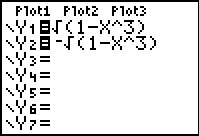
\includegraphics[width=2in]{./RelationsandFunctionsGraphics/IntrotoFunctions01.jpg} & \hspace{.75in} 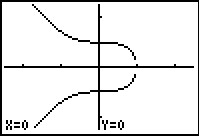
\includegraphics[width=2in]{./RelationsandFunctionsGraphics/IntrotoFunctions02.jpg} \\

\end{tabular}

\end{center}

Thus in order to use the calculator to show that $x^3 + y^2 = 1$ does not represent $y$ as a function of $x$ we needed to know \emph{analytically} that $y$ was not a function of $x$ so that we could use the calculator properly. There are more advanced graphing utilities out there which can do implicit function plots, but you need to know even more Algebra to make them work properly.  Do you get the point we're trying to make here?  We believe it is in your best interest to learn the analytic way of doing things so that you are always smarter than your calculator.

\end{ex}

\newpage

\subsection{Exercises}                                     %These are the exercises for IntrotoFunctions

In Exercises \ref{setfunctionfirst} - \ref{setfunctionlast}, determine whether or not the relation represents $y$ as a function of $x$.  Find the domain and range of those relations which are functions.

\begin{enumerate}

\item \{$(-3, 9)$, $\;(-2, 4)$, $\;(-1, 1)$, $\;(0, 0)$, $\;(1, 1)$, $\;(2, 4)$, $\;(3, 9)\}$ \label{setfunctionfirst}
\item  $\left\{ (-3,0), (1,6), (2, -3), (4,2), (-5,6), (4, -9), (6,2) \right\}$
\item  $\left\{ (-3,0), (-7,6), (5,5), (6,4), (4,9), (3,0) \right\}$
\item  $\left\{ (1,2), (4,4), (9,6), (16,8), (25,10), (36, 12), \ldots \right\}$
\item \{($x, y) \, | \, x$ is an odd integer, and $y$ is an even integer\}
\item \{$(x, 1) \, | \, x$ is an irrational number\}
\item \{$(1, 0)$, $\;(2, 1)$, $\;(4, 2)$, $\;(8, 3)$, $\;(16, 4)$, $\;(32, 5), \;$ \ldots\}
\item \{$\ldots, \; (-3, 9)$, $\;(-2, 4)$, $\;(-1, 1)$, $\;(0, 0)$, $\;(1, 1)$, $\;(2, 4)$, $\;(3, 9), \;$ \ldots\}

\setcounter{HW}{\value{enumi}}

\end{enumerate}

\begin{multicols}{2}

\begin{enumerate}

\setcounter{enumi}{\value{HW}}

\item $\{ (-2, y) \, | \, -3 < y < 4\}$
\item  $\{ (x,3) \, | \,  -2 \leq x < 4\}$

\setcounter{HW}{\value{enumi}}
\end{enumerate}
\end{multicols}

\begin{multicols}{2}
\begin{enumerate}
\setcounter{enumi}{\value{HW}}


\item  $\{ \left(x,x^2\right) \, | \, \text{$x$ is a real number} \}$
\item  $\{ \left(x^2,x\right) \, | \, \text{$x$ is a real number} \}$ \label{setfunctionlast}

\setcounter{HW}{\value{enumi}}
\end{enumerate}
\end{multicols}


In Exercises \ref{graphfunctionfirst} - \ref{graphfunctionlast}, determine whether or not the relation represents $y$ as a function of $x$.  Find the domain and range of those relations which are functions.


\begin{multicols}{2}
\begin{enumerate}
\setcounter{enumi}{\value{HW}}


\item $~$ \vspace{-.1in} \label{graphfunctionfirst}

\begin{mfpic}[17]{-5}{2}{-2}{5}
\point[3pt]{(-4, -1), (-3, 0), (-2, 1), (-1, 2), (0, 3), (1, 4)}
\axes
\tlabel[cc](2,-0.5){\scriptsize $x$}
\tlabel[cc](0.5,4.75){\scriptsize $y$}
\xmarks{-4,-3,-2,-1,1}
\ymarks{-1,1,2,3,4}
\tlpointsep{4pt}
\axislabels {x}{{\tiny $-4 \hspace{8pt}$} -4, {\tiny $-3 \hspace{8pt}$} -3, {\tiny $-2 \hspace{8pt}$} -2, {\tiny $-1 \hspace{8pt}$} -1, {\tiny $1$} 1}
\axislabels {y}{{\tiny $-1$} -1, {\tiny $1$} 1, {\tiny $2$} 2, {\tiny $3$} 3, {\tiny $4$} 4}
\end{mfpic}

\vfill
\columnbreak

\item $~$

\begin{mfpic}[15]{-5}{2}{-2}{5}
\point[3pt]{(-4, -1), (-3, 0), (-3, 1), (-2, 1), (-1, 2), (0, 3), (1, 4)}
\axes
\tlabel[cc](2,-0.5){\scriptsize $x$}
\tlabel[cc](0.5,4.75){\scriptsize $y$}
\xmarks{-4,-3,-2,-1,1}
\ymarks{-1,1,2,3,4}
\tlpointsep{4pt}
\axislabels {x}{{\tiny $-4 \hspace{6pt}$} -4, {\tiny $-3 \hspace{6pt}$} -3, {\tiny $-2 \hspace{6pt}$} -2, {\tiny $-1 \hspace{6pt}$} -1, {\tiny $1$} 1}
\axislabels {y}{{\tiny $-1$} -1, {\tiny $1$} 1, {\tiny $2$} 2, {\tiny $3$} 3, {\tiny $4$} 4}
\end{mfpic}


\setcounter{HW}{\value{enumi}}
\end{enumerate}
\end{multicols}

\pagebreak

\begin{multicols}{2}
\begin{enumerate}
\setcounter{enumi}{\value{HW}}


\item $~$

\begin{mfpic}[15]{-3}{3}{-1}{6}
\axes
\tlabel[cc](3,-0.5){\scriptsize $x$}
\tlabel[cc](0.5,5.75){\scriptsize $y$}
\xmarks{-2,-1,1,2}
\ymarks{1,2,3,4,5}
\tlpointsep{4pt}
\axislabels {x}{{\tiny $-2 \hspace{8pt}$} -2, {\tiny $-1 \hspace{8pt}$} -1, {\tiny $1$} 1, {\tiny $2$} 2}
\axislabels {y}{{\tiny $1$} 1, {\tiny $2$} 2, {\tiny $3$} 3, {\tiny $4$} 4, {\tiny $5$} 5}
\arrow \reverse \arrow \function{-2.1, 2.1, 0.1}{x**2+1}
\end{mfpic}

\vfill
\columnbreak

\item $~$

\begin{mfpic}[15]{-4}{4}{-4}{4}
\axes
\tlabel[cc](4,-0.5){\scriptsize $x$}
\tlabel[cc](0.5,3.75){\scriptsize $y$}
\xmarks{-3,-2,-1,1,2,3}
\ymarks{-3,-2,-1,1,2,3}
\tlpointsep{4pt}
\axislabels {x}{{\tiny $-3 \hspace{8pt}$} -3, {\tiny $-2 \hspace{8pt}$} -2, {\tiny $-1 \hspace{8pt}$} -1, {\tiny $1$} 1, {\tiny $2$} 2, {\tiny $3$} 3}
\axislabels {y}{{\tiny $-3$} -3, {\tiny $-2$} -2, {\tiny $-1$} -1, {\tiny $1$} 1, {\tiny $2$} 2, {\tiny $3$} 3}
\arrow \reverse \arrow \parafcn{-2,2,0.1}{(cosh(t),sinh(t))}
\arrow \reverse \arrow \parafcn{-2,2,0.1}{(-cosh(t),sinh(t))}
\end{mfpic}


\setcounter{HW}{\value{enumi}}
\end{enumerate}
\end{multicols}



\begin{multicols}{2}
\begin{enumerate}
\setcounter{enumi}{\value{HW}}

\item $~$

\begin{mfpic}[15]{-1}{10}{-1}{4}
\axes
\tlabel[cc](10,-0.5){\scriptsize $x$}
\tlabel[cc](0.5,3.75){\scriptsize $y$}
\xmarks{1,2,3,4,5,6,7,8,9}
\ymarks{1,2,3}
\tlpointsep{4pt}
\axislabels {x}{{\tiny $1$} 1, {\tiny $2$} 2, {\tiny $3$} 3, {\tiny $4$} 4, {\tiny $5$} 5, {\tiny $6$} 6, {\tiny $7$} 7, {\tiny $8$} 8, {\tiny $9$} 9}
\axislabels {y}{{\tiny $1$} 1, {\tiny $2$} 2, {\tiny $3$} 3}
\arrow \function{2, 10, 0.1}{sqrt(x - 2)}
\point[3pt]{(2,0)}
\end{mfpic}

\vfill
\columnbreak

\item $~$

\begin{mfpic}[15]{-5}{5}{-1}{5}
\axes
\tlabel[cc](5,-0.5){\scriptsize $x$}
\tlabel[cc](0.5,4.75){\scriptsize $y$}
\xmarks{-4,-3,-2,-1,1,2,3,4}
\ymarks{1,2,3,4}
\tlpointsep{4pt}
\axislabels {x}{{\tiny $-4 \hspace{8pt}$} -4, {\tiny $-3 \hspace{8pt}$} -3, {\tiny $-2 \hspace{8pt}$} -2, {\tiny $-1 \hspace{8pt}$} -1, {\tiny $1$} 1, {\tiny $2$} 2, {\tiny $3$} 3, {\tiny $4$} 4}
\axislabels {y}{{\tiny $1$} 1, {\tiny $2$} 2, {\tiny $3$} 3, {\tiny $4$} 4}
\arrow \reverse \arrow \function{-5, 5, 0.1}{4/(x**2 + 1)}
\end{mfpic}


\setcounter{HW}{\value{enumi}}
\end{enumerate}
\end{multicols}

\begin{multicols}{2}
\begin{enumerate}
\setcounter{enumi}{\value{HW}}

\item $~$


\begin{mfpic}[17]{-4.5}{5.5}{-4}{3}
\fillcolor[gray]{.7}
\gfill \rect{(-3.97, -2.97), (4.97, 1.97)}
\dashed \polyline{(-4, -3), (-4, 2)}
\dashed \polyline{(-4, 2), (5, 2)}
\dashed \polyline{(5, 2), (5, -3)}
\dashed \polyline{(5, -3), (-4, -3)}
\axes
\tlabel[cc](5.5,-0.5){\scriptsize $x$}
\tlabel[cc](0.5,2.75){\scriptsize $y$}
\xmarks{-4,-3,-2,-1,1,2,3,4,5}
\ymarks{-3,-2,-1,1,2}
\tlpointsep{4pt}
\axislabels {x}{{\tiny $-4 \hspace{8pt}$} -4, {\tiny $-3 \hspace{8pt}$} -3, {\tiny $-2 \hspace{8pt}$} -2, {\tiny $-1 \hspace{8pt}$} -1, {\tiny $1$} 1, {\tiny $2$} 2, {\tiny $3$} 3, {\tiny $4$} 4, {\tiny $5$} 5}
\axislabels {y}{{\tiny $-3$} -3, {\tiny $-2$} -2, {\tiny $-1$} -1, {\tiny $1$} 1, {\tiny $2$} 2}
\end{mfpic}

\vfill
\columnbreak

\item $~$

\begin{mfpic}[15]{-6}{4}{-3}{5}
\function{-5,-1,0.1}{-5 - 6*x - x**2}
\function{-1,3,0.1}{x/4 - 7/4}
\point[3pt]{(-5, 0), (-1, 0)}
\gclear \circle{(-3,4), 0.1}
\circle{(-3,4), 0.1}
\gclear \circle{(-1,-2), 0.1}
\circle{(-1,-2), 0.1}
\gclear \circle{(3,-1), 0.1}
\circle{(3,-1), 0.1}
\axes
\tlabel[cc](4,-0.5){\scriptsize $x$}
\tlabel[cc](0.5,4.75){\scriptsize $y$}
\xmarks{-5 step 1 until 3}
\ymarks{-2 step 1 until 4}
\tlpointsep{4pt}
\axislabels {x}{{\tiny $-5 \hspace{8pt}$} -5, {\tiny $-4 \hspace{8pt}$} -4, {\tiny $-3 \hspace{8pt}$} -3, {\tiny $-2 \hspace{8pt}$} -2, {\tiny $-1 \hspace{8pt}$} -1, {\tiny $1$} 1, {\tiny $2$} 2, {\tiny $3$} 3}
\axislabels {y}{{\tiny $-2$} -2, {\tiny $-1$} -1, {\tiny $1$} 1, {\tiny $2$} 2, {\tiny $3$} 3, {\tiny $4$} 4}
\end{mfpic}


\setcounter{HW}{\value{enumi}}
\end{enumerate}
\end{multicols}

\begin{multicols}{2}
\begin{enumerate}
\setcounter{enumi}{\value{HW}}

\item  $~$

\begin{mfpic}[8]{-4}{4}{-6}{10}
\point[3pt]{(-2,6), (1,-3) }
\axes
\tlabel[cc](4,-0.5){\scriptsize $x$}
\tlabel[cc](0.5,10){\scriptsize $y$}
\xmarks{-3,-2,-1,1,2,3}
\ymarks{-5,-4,-3,-2,-1,1,2,3,4,5,6,7,8,9}
\tlpointsep{4pt}
\axislabels {x}{{\tiny $-3 \hspace{6pt}$} -3,{\tiny $-2 \hspace{6pt}$} -2, {\tiny $-1 \hspace{6pt}$} -1, {\tiny $1$} 1, {\tiny $2$} 2, {\tiny $3$} 3}
\axislabels {y}{{\tiny $-5$} -5, {\tiny $-4$} -4, {\tiny $-3$} -3, {\tiny $-2$} -2, {\tiny $-1$} -1, {\tiny $1$} 1, {\tiny $2$} 2, {\tiny $3$} 3, {\tiny $4$} 4, {\tiny $5$} 5, {\tiny $6$} 6, {\tiny $7$} 7, {\tiny $8$} 8, {\tiny $9$} 9}
\arrow \function{-2,4.5,0.1}{x**2 - 2*x - 2}
\end{mfpic}

\vfill
\columnbreak

\item  $~$

\begin{mfpic}[10]{-6}{6}{-6}{6}
\axes
\tlabel[cc](6,-0.5){\scriptsize $x$}
\tlabel[cc](0.5,6){\scriptsize $y$}
\xmarks{-5,-4,-3,-2,-1,1,2,3,4,5}
\ymarks{-5,-4,-3,-2,-1,1,2,3,4,5}
\tlpointsep{4pt}
\axislabels {x}{{\tiny $-5 \hspace{6pt}$} -5,{\tiny $-4 \hspace{6pt}$} -4,{\tiny $-3 \hspace{6pt}$} -3,{\tiny $-2 \hspace{6pt}$} -2, {\tiny $-1 \hspace{6pt}$} -1, {\tiny $1$} 1, {\tiny $2$} 2, {\tiny $3$} 3, {\tiny $4$} 4, {\tiny $5$} 5}
\axislabels {y}{{\tiny $-5$} -5,{\tiny $-4$} -4,{\tiny $-3$} -3, {\tiny $-2$} -2, {\tiny $-1$} -1, {\tiny $1$} 1, {\tiny $2$} 2, {\tiny $3$} 3, {\tiny $4$} 4, {\tiny $5$} 5}
\plrfcn{0,180,5}{5*sind 3t}
\end{mfpic} 


\setcounter{HW}{\value{enumi}}
\end{enumerate}
\end{multicols}

\begin{multicols}{2}
\begin{enumerate}
\setcounter{enumi}{\value{HW}}

\item  $~$

\begin{mfpic}[10]{-6}{6}{-6}{6}
\axes
\tlabel[cc](6,-0.5){\scriptsize $x$}
\tlabel[cc](0.5,6){\scriptsize $y$}
\xmarks{-5,-4,-3,-2,-1,1,2,3,4,5}
\ymarks{-5,-4,-3,-2,-1,1,2,3,4,5}
\tlpointsep{4pt}
\axislabels {x}{{\tiny $-5 \hspace{6pt}$} -5,{\tiny $-4 \hspace{6pt}$} -4,{\tiny $-3 \hspace{6pt}$} -3,{\tiny $-2 \hspace{6pt}$} -2, {\tiny $-1 \hspace{6pt}$} -1, {\tiny $1$} 1, {\tiny $2$} 2, {\tiny $3$} 3, {\tiny $4$} 4, {\tiny $5$} 5}
\axislabels {y}{{\tiny $-5$} -5,{\tiny $-4$} -4,{\tiny $-3$} -3, {\tiny $-2$} -2, {\tiny $-1$} -1, {\tiny $1$} 1, {\tiny $2$} 2, {\tiny $3$} 3, {\tiny $4$} 4, {\tiny $5$} 5}
\function{-5,4,0.1}{0.0502*(x**3) - 0.0344*(x**2) - 0.2010*x + 2.138}
\gfill \circle{(-5,-4),0.2}
\gclear \circle{(4,4),0.2}
\circle{(4,4),0.2}
\end{mfpic} 

\vfill
\columnbreak

\item  $~$

\begin{mfpic}[10]{-2}{7}{-6}{6}
\axes
\tlabel[cc](7,-0.5){\scriptsize $x$}
\tlabel[cc](0.5,6){\scriptsize $y$}
\xmarks{-1,1,2,3,4,5,6}
\ymarks{-5,-4,-3,-2,-1,1,2,3,4,5}
\tlpointsep{4pt}
\axislabels {x}{{\tiny $-1 \hspace{6pt}$} -1, {\tiny $1$} 1, {\tiny $2$} 2, {\tiny $3$} 3, {\tiny $4$} 4, {\tiny $5$} 5, {\tiny $6$} 6}
\axislabels {y}{{\tiny $-5$} -5,{\tiny $-4$} -4,{\tiny $-3$} -3, {\tiny $-2$} -2, {\tiny $-1$} -1, {\tiny $1$} 1, {\tiny $2$} 2, {\tiny $3$} 3, {\tiny $4$} 4, {\tiny $5$} 5}
\polyline{(0,-1), (3,-4)}
\polyline{(3,1), (4,4), (6,0)}
\point[3pt]{(0,-1), (4,4), (6,0)}
\pointfillfalse
\point[3pt]{(3,-4), (3,1)}
\end{mfpic} 

\setcounter{HW}{\value{enumi}}
\end{enumerate}
\end{multicols}

\begin{multicols}{2}
\begin{enumerate}
\setcounter{enumi}{\value{HW}}

\item  $~$

\begin{mfpic}[15]{-3}{3}{-1}{5}
\axes
\tlabel[cc](3,-0.5){\scriptsize $x$}
\tlabel[cc](0.5,5){\scriptsize $y$}
\xmarks{-2,-1,1,2}
\ymarks{1,2,3,4}
\tlpointsep{4pt}
\axislabels {x}{{\tiny $-2 \hspace{6pt}$} -2, {\tiny $-1 \hspace{6pt}$} -1, {\tiny $1$} 1, {\tiny $2$} 2}
\axislabels {y}{{\tiny $1$} 1, {\tiny $2$} 2, {\tiny $3$} 3, {\tiny $4$} 4}
\arrow \reverse \arrow \function{-2.25,2.25,0.1}{4-(x**2)}
\end{mfpic} 

\vfill
\columnbreak

\item  $~$


\begin{mfpic}[15]{-3}{3}{-1}{5}
\axes
\tlabel[cc](3,-0.5){\scriptsize $x$}
\tlabel[cc](0.5,5){\scriptsize $y$}
\xmarks{-2,-1,1,2}
\ymarks{1,2,3,4}
\tlpointsep{4pt}
\axislabels {x}{{\tiny $-2 \hspace{6pt}$} -2, {\tiny $-1 \hspace{6pt}$} -1, {\tiny $1$} 1, {\tiny $2$} 2}
\axislabels {y}{{\tiny $1$} 1, {\tiny $2$} 2, {\tiny $3$} 3, {\tiny $4$} 4}
\arrow \reverse \arrow \polyline{(-2,-1), (1,4), (2,-1)}
\end{mfpic} 

\setcounter{HW}{\value{enumi}}
\end{enumerate}
\end{multicols}

\begin{multicols}{2}
\begin{enumerate}
\setcounter{enumi}{\value{HW}}

\item  $~$

\begin{mfpic}[15]{-3}{3}{-1}{5}
\axes
\tlabel[cc](3,-0.5){\scriptsize $x$}
\tlabel[cc](0.5,5){\scriptsize $y$}
\xmarks{-2,-1,1,2}
\ymarks{1,2,3,4}
\tlpointsep{4pt}
\axislabels {x}{{\tiny $-2 \hspace{6pt}$} -2, {\tiny $-1 \hspace{6pt}$} -1, {\tiny $1$} 1, {\tiny $2$} 2}
\axislabels {y}{{\tiny $1$} 1, {\tiny $2$} 2, {\tiny $3$} 3, {\tiny $4$} 4}
\arrow \function{-2, 2, 0.1}{3-2*sqrt(x+2)}
\point[3pt]{(-2,3)}
\end{mfpic} 

\vfill
\columnbreak

\item  $~$


\begin{mfpic}[15]{-3}{3}{-1}{5}
\axes
\tlabel[cc](3,-0.5){\scriptsize $x$}
\tlabel[cc](0.5,5){\scriptsize $y$}
\xmarks{-2,-1,1,2}
\ymarks{1,2,3,4}
\tlpointsep{4pt}
\axislabels {x}{{\tiny $-2 \hspace{6pt}$} -2, {\tiny $-1 \hspace{6pt}$} -1, {\tiny $1$} 1, {\tiny $2$} 2}
\axislabels {y}{{\tiny $1$} 1, {\tiny $2$} 2, {\tiny $3$} 3, {\tiny $4$} 4}
\arrow \reverse \arrow \function{-2.25, 1.75, 0.1}{x*(x-1)*(x+2)}
\end{mfpic} 

\setcounter{HW}{\value{enumi}}
\end{enumerate}
\end{multicols}

\begin{multicols}{2}
\begin{enumerate}
\setcounter{enumi}{\value{HW}}

\item  $~$

\begin{mfpic}[15]{-3}{3}{-3}{3}
\axes
\tlabel[cc](3,-0.5){\scriptsize $x$}
\tlabel[cc](0.5,3){\scriptsize $y$}
\xmarks{-2,-1,1,2}
\ymarks{-2,-1,1,2}
\tlpointsep{4pt}
\axislabels {x}{{\tiny $-2 \hspace{6pt}$} -2, {\tiny $-1 \hspace{6pt}$} -1, {\tiny $1$} 1, {\tiny $2$} 2}
\axislabels {y}{{\tiny $1$} 1, {\tiny $2$} 2, {\tiny $-2$} -2, {\tiny $-1$} -1}
\arrow \polyline{(0,1), (-2,-2)}
\arrow \polyline{(1,2), (3,2)}
\point[3pt]{(0,1)}
\pointfillfalse
\point[3pt]{(1,2)}
\end{mfpic} 

\vfill
\columnbreak

\item  $~$


\begin{mfpic}[15]{-4}{4}{-3}{3}
\axes
\tlabel[cc](4,-0.5){\scriptsize $x$}
\tlabel[cc](0.5,3){\scriptsize $y$}
\xmarks{-3,-2,-1,1,2,3}
\ymarks{-2,-1,1,2}
\tlpointsep{4pt}
\axislabels {x}{{\tiny $-3 \hspace{6pt}$} -3,{\tiny $-2 \hspace{6pt}$} -2, {\tiny $-1 \hspace{6pt}$} -1, {\tiny $1$} 1, {\tiny $2$} 2, {\tiny $3$} 3}
\axislabels {y}{{\tiny $1$} 1, {\tiny $2$} 2, {\tiny $-2$} -2, {\tiny $-1$} -1}
\function{-3,3,0.1}{2*sin(1.05*x)}
\point[3pt]{(-3,0)}
\point[3pt]{(3,0)}
\end{mfpic} 

\setcounter{HW}{\value{enumi}}
\end{enumerate}
\end{multicols}

\pagebreak

\begin{multicols}{2}
\begin{enumerate}
\setcounter{enumi}{\value{HW}}

\item  $~$

\begin{mfpic}[15]{-3}{3}{-3}{3}
\axes
\tlabel[cc](3,-0.5){\scriptsize $x$}
\tlabel[cc](0.5,3){\scriptsize $y$}
\xmarks{-2,-1,1,2}
\ymarks{-2,-1,1,2}
\tlpointsep{4pt}
\axislabels {x}{{\tiny $-2 \hspace{6pt}$} -2, {\tiny $-1 \hspace{6pt}$} -1, {\tiny $1$} 1, {\tiny $2$} 2}
\axislabels {y}{{\tiny $1$} 1, {\tiny $2$} 2, {\tiny $-2$} -2, {\tiny $-1$} -1}
\arrow \reverse \arrow \polyline{(2,-3), (2,3)}
\end{mfpic} 

\vfill
\columnbreak

\item  $~$ \label{graphfunctionlast}


\begin{mfpic}[15]{-3}{3}{-3}{3}
\axes
\tlabel[cc](3,-0.5){\scriptsize $x$}
\tlabel[cc](0.5,3){\scriptsize $y$}
\xmarks{-2,-1,1,2}
\ymarks{-2,-1,1,2}
\tlpointsep{4pt}
\axislabels {x}{{\tiny $-2 \hspace{6pt}$} -2, {\tiny $-1 \hspace{6pt}$} -1, {\tiny $1$} 1, {\tiny $2$} 2}
\axislabels {y}{{\tiny $1$} 1, {\tiny $2$} 2, {\tiny $-2$} -2, {\tiny $-1$} -1}
\arrow \reverse \arrow \polyline{(-3,2), (3,2)}
\end{mfpic} 

\setcounter{HW}{\value{enumi}}
\end{enumerate}
\end{multicols}

In Exercises \ref{equfunctionfirst} - \ref{equfunctionlast}, determine whether or not the equation represents $y$ as a function of $x$.

\begin{multicols}{3}
\begin{enumerate}
\setcounter{enumi}{\value{HW}}

\item $y = x^{3} - x$ \label{equfunctionfirst}
\item $y = \sqrt{x - 2}$
\item $x^{3}y = -4$ 
\setcounter{HW}{\value{enumi}}
\end{enumerate}
\end{multicols}

\begin{multicols}{3}
\begin{enumerate}
\setcounter{enumi}{\value{HW}}

\item $x^{2} - y^{2} = 1$
\item $y = \dfrac{x}{x^{2} - 9}$
\item $x = -6$

\setcounter{HW}{\value{enumi}}
\end{enumerate}
\end{multicols}

\begin{multicols}{3}
\begin{enumerate}
\setcounter{enumi}{\value{HW}}

\item  $x = y^2 + 4$

\item $y = x^2 + 4$
\item $x^2 + y^2 = 4$

\setcounter{HW}{\value{enumi}}
\end{enumerate}
\end{multicols}

\begin{multicols}{3}
\begin{enumerate}
\setcounter{enumi}{\value{HW}}


\item $y = \sqrt{4-x^2}$
\item $x^2 - y^2 = 4$
\item $x^3 + y^3 = 4$


\setcounter{HW}{\value{enumi}}
\end{enumerate}
\end{multicols}

\begin{multicols}{3}
\begin{enumerate}
\setcounter{enumi}{\value{HW}}

\item $2x + 3y = 4$
\item $2xy = 4$
\item $x^2 = y^2$ \label{equfunctionlast}

\setcounter{HW}{\value{enumi}}
\end{enumerate}
\end{multicols}

\begin{enumerate}
\setcounter{enumi}{\value{HW}}

\item Explain why the population $P$ of Sasquatch in a given area is a function of time $t$.  What would be the range of this function?

\item Explain why the relation between your classmates and their email addresses may not be a function.  What about phone numbers and Social Security Numbers?

\setcounter{HW}{\value{enumi}}
\end{enumerate}

The process given in Example \hspace{-.1in} ~\ref{introfunctionlastexample} for determining whether an equation of a relation represents $y$ as a function of $x$ breaks down if we cannot solve the equation for $y$ in terms of $x$.  However, that does not prevent us from proving that an equation fails to represent $y$ as a function of $x$.  What we really need is two points with the same $x$-coordinate and different $y$-coordinates which both satisfy the equation so that the graph of the relation would fail the Vertical Line Test \hspace{-.1in} ~\ref{VLT}.  Discuss with your classmates how you might find such points for the relations given in Exercises \ref{notfuncequfirst} - \ref{notfuncequlast}.

\begin{multicols}{2}
\begin{enumerate}
\setcounter{enumi}{\value{HW}}

\item $x^{3} + y^{3} - 3xy = 0$ \label{notfuncequfirst}
\item $x^{4} = x^{2} + y^{2}$ 

\setcounter{HW}{\value{enumi}}
\end{enumerate}
\end{multicols}

\begin{multicols}{2}
\begin{enumerate}
\setcounter{enumi}{\value{HW}}


\item $y^{2} = x^{3} + 3x^{2}$ 
\item $(x^{2} + y^{2})^{2} = x^{3} + y^{3}$ \label{notfuncequlast}

\setcounter{HW}{\value{enumi}}
\end{enumerate}
\end{multicols}

\newpage

\subsection{Answers}

\begin{multicols}{2}
\begin{enumerate}

\item Function \\ domain = \{$-3$, $-2$, $-1$, $0$, $1$, $2$ ,$3$\} \\ range = \{$0$, $1$, $4$, $9$\}

\vfill

\columnbreak

\item Not a function

\setcounter{HW}{\value{enumi}}
\end{enumerate}
\end{multicols}

\begin{multicols}{2}
\begin{enumerate}
\setcounter{enumi}{\value{HW}}

\item  Function \\ domain = $\left\{ -7, -3, 3, 4, 5, 6 \right\}$ \\ range = $\left\{ 0,4,5,6,9 \right\}$


\vfill

\columnbreak

\item  Function \\ domain =   $\left\{ 1, 4, 9, 16, 25, 36, \ldots \right\} \\ = \left\{ x \, | \, \text{$x$ is a perfect square} \right\}$ \\ range =  $\left\{ 2, 4, 6, 8, 10, 12, \ldots \right\} \\ = \left\{ y \, | \, \text{$y$ is a positive even integer} \right\}$

\setcounter{HW}{\value{enumi}}
\end{enumerate}
\end{multicols}

\begin{multicols}{2}
\begin{enumerate}
\setcounter{enumi}{\value{HW}}

\item  Not a function

\vfill

\columnbreak

\item Function \\ domain = \{$x$ \, | \, $x$ is irrational\} \\ range = \{$1$\}

\setcounter{HW}{\value{enumi}}
\end{enumerate}
\end{multicols}

\begin{multicols}{2}
\begin{enumerate}
\setcounter{enumi}{\value{HW}}

\item Function \\ domain = \{$x$ \, | \, $x = 2^{n}$ for some whole number $n$\} \\ range = \{$y$ \, | \, $y$ is any whole number\}

\vfill

\columnbreak

\item Function \\ domain = \{$x$ \, | \, $x$ is any integer\} \\ range = \{$y$ \, | \, $y = n^{2}$ for some integer $n$\}

\setcounter{HW}{\value{enumi}}
\end{enumerate}
\end{multicols}

\begin{multicols}{2}
\begin{enumerate}
\setcounter{enumi}{\value{HW}}

\item Not a function

\vfill

\columnbreak

\item Function \\ domain = $[-2, 4)$, range = \{$3$\}

\setcounter{HW}{\value{enumi}}
\end{enumerate}
\end{multicols}

\begin{multicols}{2}
\begin{enumerate}
\setcounter{enumi}{\value{HW}}


\item Function \\ domain = $(-\infty, \infty)$ \\  range = $[0,\infty)$

\vfill

\columnbreak

\item  Not a function

\setcounter{HW}{\value{enumi}}
\end{enumerate}
\end{multicols}

\begin{multicols}{2}
\begin{enumerate}
\setcounter{enumi}{\value{HW}}

\item Function \\ domain = \{$-4$, $-3$, $-2$, $-1$, $0$, $1$\} \\ range = \{$-1$, $0$, $1$, $2$, $3$, $4$\}

\vfill

\columnbreak

\item Not a function

\setcounter{HW}{\value{enumi}}
\end{enumerate}
\end{multicols}


\begin{multicols}{2}
\begin{enumerate}
\setcounter{enumi}{\value{HW}}

\item Function \\ domain = $(-\infty, \infty)$ \\ range = $[1, \infty)$

\vfill

\columnbreak

\item Not a function

\setcounter{HW}{\value{enumi}}
\end{enumerate}
\end{multicols}


\begin{multicols}{2}
\begin{enumerate}
\setcounter{enumi}{\value{HW}}

\item Function \\ domain = $[2, \infty)$ \\ range = $[0, \infty)$

\vfill

\columnbreak

\item Function \\ domain = $(-\infty, \infty)$ \\ range = $(0, 4]$

\setcounter{HW}{\value{enumi}}
\end{enumerate}
\end{multicols}


\begin{multicols}{2}
\begin{enumerate}
\setcounter{enumi}{\value{HW}}

\item Not a function


\vfill

\columnbreak

\item Function \\ domain = $[-5,-3) \cup(-3, 3)$ \\ range = $(-2, -1) \cup [0, 4)$

\setcounter{HW}{\value{enumi}}
\end{enumerate}
\end{multicols}


\begin{multicols}{2}
\begin{enumerate}
\setcounter{enumi}{\value{HW}}

\item  Function \\  domain =  $[-2, \infty)$ \\ range = $[-3, \infty)$

\vfill

\columnbreak

\item Not a function

\setcounter{HW}{\value{enumi}}
\end{enumerate}
\end{multicols}


\begin{multicols}{2}
\begin{enumerate}
\setcounter{enumi}{\value{HW}}

\item  Function \\  domain =  $[-5,4)$ \\ range =  $[-4,4)$

\vfill

\columnbreak

\item  Function \\ domain = $[0,3) \cup (3,6]$ \\ range = $(-4,-1] \cup [0,4]$

\setcounter{HW}{\value{enumi}}
\end{enumerate}
\end{multicols}


\begin{multicols}{2}
\begin{enumerate}
\setcounter{enumi}{\value{HW}}

\item  Function \\  domain =  $(-\infty, \infty)$ \\ range =  $(-\infty, 4]$

\vfill

\columnbreak

\item  Function \\ domain = $(-\infty, \infty)$ \\ range = $(-\infty, 4]$

\setcounter{HW}{\value{enumi}}
\end{enumerate}
\end{multicols}


\begin{multicols}{2}
\begin{enumerate}
\setcounter{enumi}{\value{HW}}

\item  Function \\  domain =  $[-2, \infty)$ \\ range =  $(-\infty, 3]$

\vfill

\columnbreak

\item  Function \\ domain = $(-\infty, \infty)$ \\ range = $(-\infty, \infty)$

\setcounter{HW}{\value{enumi}}
\end{enumerate}
\end{multicols}


\begin{multicols}{2}
\begin{enumerate}
\setcounter{enumi}{\value{HW}}

\item  Function \\  domain =  $(-\infty, 0] \cup (1, \infty)$ \\ range =  $(-\infty, 1] \cup \{ 2\}$

\vfill

\columnbreak

\item  Function \\ domain = $[-3,3]$ \\ range = $[-2,2]$

\setcounter{HW}{\value{enumi}}
\end{enumerate}
\end{multicols}

\begin{multicols}{2}
\begin{enumerate}
\setcounter{enumi}{\value{HW}}

\item  Not a function

\vfill

\columnbreak

\item  Function \\ domain = $(-\infty, \infty)$ \\ range = $\{2\}$

\setcounter{HW}{\value{enumi}}
\end{enumerate}
\end{multicols}



\begin{multicols}{3}
\begin{enumerate}
\setcounter{enumi}{\value{HW}}


\item Function
\item Function
\item Function

\setcounter{HW}{\value{enumi}}
\end{enumerate}
\end{multicols}

\begin{multicols}{3}
\begin{enumerate}
\setcounter{enumi}{\value{HW}}


\item Not a function
\item Function
\item Not a function

\setcounter{HW}{\value{enumi}}
\end{enumerate}
\end{multicols}

\begin{multicols}{3}
\begin{enumerate}
\setcounter{enumi}{\value{HW}}

\item  Not a function
\item  Function
\item  Not a function

\setcounter{HW}{\value{enumi}}
\end{enumerate}
\end{multicols}

\begin{multicols}{3}
\begin{enumerate}
\setcounter{enumi}{\value{HW}}

\item   Function
\item   Not a function
\item Function

\setcounter{HW}{\value{enumi}}
\end{enumerate}
\end{multicols}

\begin{multicols}{3}
\begin{enumerate}
\setcounter{enumi}{\value{HW}}

\item Function
\item  Function
\item Not a function

\setcounter{HW}{\value{enumi}}
\end{enumerate}
\end{multicols}
\closegraphsfile